% THIS IS SIGPROC-SP.TEX - VERSION 3.1
% WORKS WITH V3.2SP OF ACM_PROC_ARTICLE-SP.CLS
% APRIL 2009
%
% It is an example file showing how to use the 'acm_proc_article-sp.cls' V3.2SP
% LaTeX2e document class file for Conference Proceedings submissions.
% ----------------------------------------------------------------------------------------------------------------
% This .tex file (and associated .cls V3.2SP) *DOES NOT* produce:
%       1) The Permission Statement
%       2) The Conference (location) Info information
%       3) The Copyright Line with ACM data
%       4) Page numbering
% ---------------------------------------------------------------------------------------------------------------
% It is an example which *does* use the .bib file (from which the .bbl file
% is produced).
% REMEMBER HOWEVER: After having produced the .bbl file,
% and prior to final submission,
% you need to 'insert'  your .bbl file into your source .tex file so as to provide
% ONE 'self-contained' source file.
%
% Questions regarding SIGS should be sent to
% Adrienne Griscti ---> griscti@acm.org
%
% Questions/suggestions regarding the guidelines, .tex and .cls files, etc. to
% Gerald Murray ---> murray@hq.acm.org
%
% For tracking purposes - this is V3.1SP - APRIL 2009

\documentclass{acm_proc_article-sp}
\usepackage{ctex}[utf8]
\usepackage{float}
\usepackage{listings}
\begin{document}

\title{实验报告:迷宫寻路AI}
%
% You need the command \numberofauthors to handle the 'placement
% and alignment' of the authors beneath the title.
%
% For aesthetic reasons, we recommend 'three authors at a time'
% i.e. three 'name/affiliation blocks' be placed beneath the title.
%
% NOTE: You are NOT restricted in how many 'rows' of
% "name/affiliations" may appear. We just ask that you restrict
% the number of 'columns' to three.
%
% Because of the available 'opening page real-estate'
% we ask you to refrain from putting more than six authors
% (two rows with three columns) beneath the article title.
% More than six makes the first-page appear very cluttered indeed.
%
% Use the \alignauthor commands to handle the names
% and affiliations for an 'aesthetic maximum' of six authors.
% Add names, affiliations, addresses for
% the seventh etc. author(s) as the argument for the
% \additionalauthors command.
% These 'additional authors' will be output/set for you
% without further effort on your part as the last section in
% the body of your article BEFORE References or any Appendices.

\numberofauthors{2} %  in this sample file, there are a *total*
% of EIGHT authors. SIX appear on the 'first-page' (for formatting
% reasons) and the remaining two appear in the \additionalauthors section.
%
\author{
% You can go ahead and credit any number of authors here,
% e.g. one 'row of three' or two rows (consisting of one row of three
% and a second row of one, two or three).
%
% The command \alignauthor (no curly braces needed) should
% precede each author name, affiliation/snail-mail address and
% e-mail address. Additionally, tag each line of
% affiliation/address with \affaddr, and tag the
% e-mail address with \email.
%
% 1st. author
\alignauthor
郑炜熹 \\
软72 \\
2016013170 
% 2nd. author
\alignauthor
曾正 \\
软71 \\
2017011438
}
% There's nothing stopping you putting the seventh, eighth, etc.
% author on the opening page (as the 'third row') but we ask,
% for aesthetic reasons that you place these 'additional authors'
% in the \additional authors block, viz.

% Just remember to make sure that the TOTAL number of authors
% is the number that will appear on the first page PLUS the
% number that will appear in the \additionalauthors section.

\maketitle
\begin{abstract}
本次实验报告介绍了Markov决策过程以及其描述, 迷宫寻路AI程序的python实现以及实验结果.
\end{abstract}

\keywords{Markov Decision Process} % NOT required for Proceedings

\section{算法简介}

Markov决策过程有以下元素:
\begin{itemize}
    \item 状态集合$S$.
    \item 动作集合$A$.
    \item 初始状态$s_0$.
    \item 结束状态集合$\{s_f\}$.
    \item 动作策略$\pi$.
\end{itemize}

有以下函数:
\begin{itemize}
    \item 后继概率函数$P(s, a, s^\prime)$: 状态$s$执行动作$a$后转移到状态$s^\prime$的概率.
    \item 回报函数$R(s, a, s^\prime)$: 状态$s$执行动作$a$后转移到状态$s^\prime$后获得的回报值.
    \item 行为价值函数$Q_\pi(s, a)$, 表示在执行策略$\pi$时, 对当前状态$s$执行某一具体行为$a$所能得到的回报值期望.
    \item 状态价值函数$V_\pi(s)$, 表示某一状态在策略$\pi$下, 从该状态开始的马尔可夫链收获的累计回报值期望.
\end{itemize}

该决策过程目的是为了求出最优策略$\pi^*$:
$$
\pi^* = \arg \max_\pi V^\pi(s), \forall s
$$

因为对于任何MDP, 总存在确定性的最优策略, 则我们可以通过以下的迭代函数(Bellman 方程):
\begin{align}
V_{k+1}(s) \gets \max_a \sum_{s^\prime}P(s, a, s^\prime)[R(s, a, s^\prime) + \gamma V_k(s^\prime)]
\end{align}
收敛时可以求出最优的状态价值函数$V_*(s)$和行为价值函数$Q_*(s, a)$, 之后我们便可以通过:
$$
\pi^*(a|s) = 
\begin{cases}
    1, & a = \arg \max_a Q_*(s, a) \\
    0, & otherwise
\end{cases}
$$
求出确定性的最优策略.

\section{地图设计和算法实例化}

对于迷宫寻路AI, 我们将地图方块分为4类:
\begin{itemize}
    \item 普通方块.
    \item 障碍方块, 当移动到该方块时会自动返回原位置.
    \item 陷阱方块, 当移动到该方块时会返回起点.
    \item 终点方块.
\end{itemize}

动作分为四类: 上, 下, 左, 右. 每个方向都有分别$1/5$的概率移动到两个对角, $3/5$的概率移动到正方向.

根据这些特点, 我们可以设置对应的$P(s, a, s^\prime)$和$R(s, a, s^\prime)$:
\begin{itemize}
    \item 当$s$通过$a$跳转的是普通方块或是终点方块, 则$s^\prime$为对应的目标普通方块位置.
    \item 当$s$通过$a$跳转的是障碍方块, 则$s^\prime$为$s$对应的位置.
    \item 当$s$通过$a$跳转的是陷阱方块, 则$s^\prime$为起点位置.
\end{itemize}
概率$P$为对应的跳转概率值, 回报$R$根据目标方块设置回报值.

本次实验回报值设置为: 陷阱和终点分别设为负值和正值, 普通方块和障碍方块设为0. 
这种策略使得AI会尽量避开陷阱和障碍物, 寻找离终点最近的道路(在$\gamma < 1$情况下).

\section{算法实现}

本算法采用python实现, 算法类为Markov, 在\textsf{Markov.py}文件中.

该类有一些比较关键的成员:
\begin{itemize}
    \item 变量\textsf{REWARD\_<type>}. 指定每种方块的回报值, 相当于回报函数.
    \item 变量\textsf{gamma}. 衰减因子.
    \item 函数\textsf{read\_map}. 读取地图信息.
    \item 函数\textsf{initialize\_state}, 根据地图和回报值设定来初始化$P$和$R$, 初始化算法的数据结构等.
    \item 函数\textsf{update\_value\_once}, 执行一次Bellman方程迭代计算, 同时求出当前迭代下的最优策略.
\end{itemize}

算法实现的关键点:
\begin{itemize}
    \item 数据结构的设计, 我们在\textsf{initialize\_state}中设置了几个变量: 
    \begin{itemize}
        \item \textsf{trans\_dist}为一个字典, 字典的每一个key都指定了一个动作(上下左右), 每个key指向一个二维
        列表, 其中第一维对应为前驱方块的位置, 二维为该前驱方框通过当前的action(也就是key对应的动作)能达到的方块的位置.
        \item \textsf{trans\_prob}与上面类似, 只不过第二维为该前驱方框通过当前的action到达在\textsf{trans\_dist}对应方块位置的概率.
        \item \textsf{reward}与上面类似, 第二维为该前驱方框通过当前的action到达在\textsf{trans\_dist}对应方块后能获得的回报值.
    \end{itemize}
    这些数据结构构成了$R(s, a, s^\prime)$和$P(s, a, s^\prime)$.相比于纯粹的矩阵, 在迭代时能节省一部分时间(因为矩阵是稀疏矩阵, 第二维的大小为所有方格的总数, 
    而这个数据结构使得第二维能减小至有概率转移到的方块的个数). 执行函数后, 这些数据结构将会根据地图初始化.
    \item 算法的实现, 我们在\textsf{update\_value\_once}执行一次Bellman公式的迭代, 具体来说便是根据当前的价值函数$V(s)$(初始为
    长度$m*n$的零向量, $m, n$分别为行列个数), 衰减因子$\gamma$, $R(s, a, s^\prime)$和$P(s, a, s^\prime)$来计算每个动作分别对应的价值, 
    然后求出最大值赋值于$V(s)$中, 同时将对应的最优动作保存于每个方块中.
\end{itemize}

\section{实验结果展示}

为了测试, 我们设计了以下的地图:
\begin{figure}[H]
    \centering
    \caption{$N=0$}
    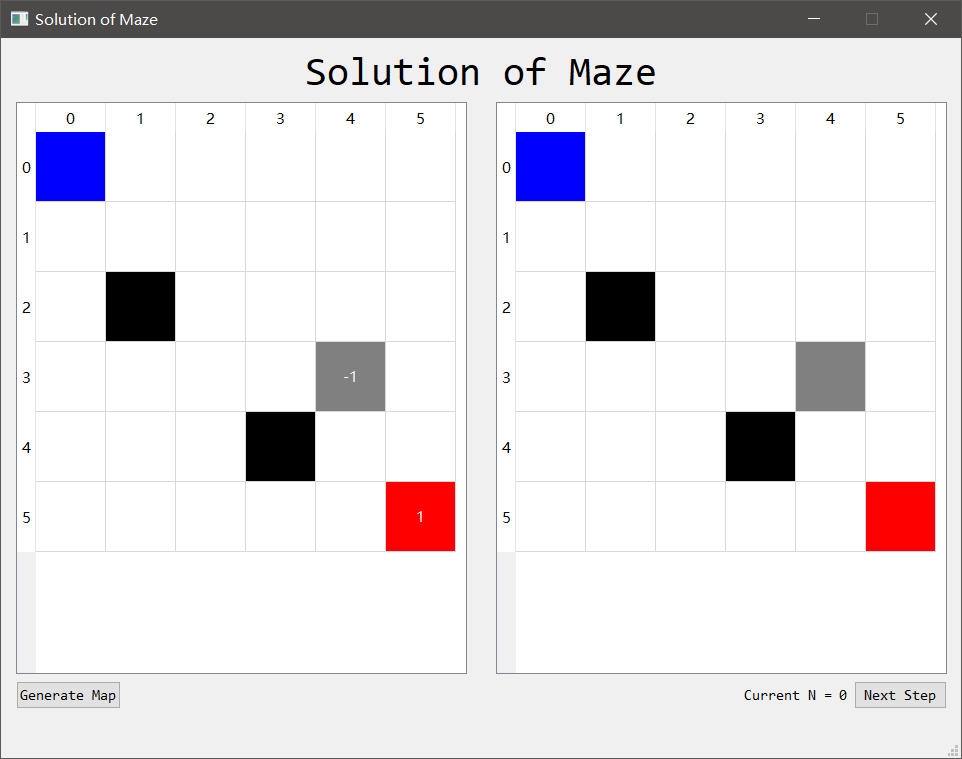
\includegraphics[width=0.4\textwidth]{figure1.png}
\end{figure}

其中蓝色方块为起点, 红色方块为终点, 黑色方块为障碍物, 灰色方块为陷阱. 本次实验$\gamma = 0.8$.
\begin{figure}[H]
    \centering
    \caption{$N=1$}
    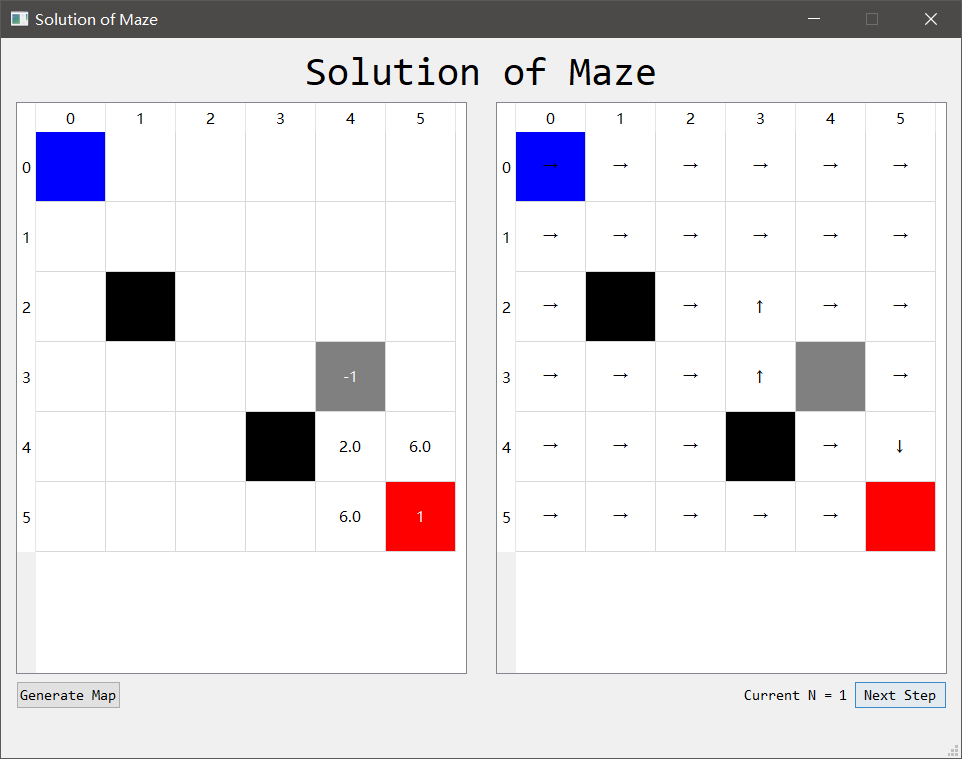
\includegraphics[width=0.4\textwidth]{figure2.png}
\end{figure}

在执行完一次迭代后, 可以看到终点周围的方块对应的价值根据迭代值更新了, 而对应右边表示的最优策略也指向了终点. 
大部分没有更新的方块价值, 其对应的最优策略是$\rightarrow$(默认值).
\begin{figure}[H]
    \centering
    \caption{$N=5$}
    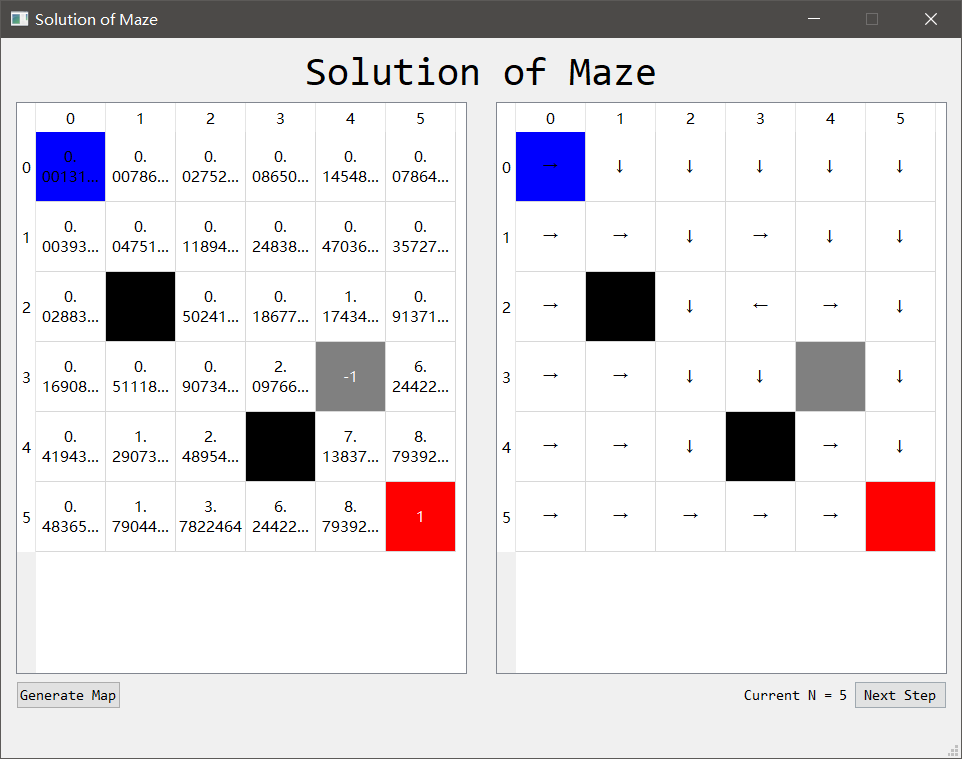
\includegraphics[width=0.4\textwidth]{figure3.png}
\end{figure}

而在执行了5次迭代后, 所有的方块的价值都被更新到非0值, 同时最优策略也被更新, 可以看到这些方向大都是朝着终点指向的.

为了获得收敛价值, 我们执行多次迭代:

\begin{figure}[H]
    \centering
    \caption{$N=30$}
    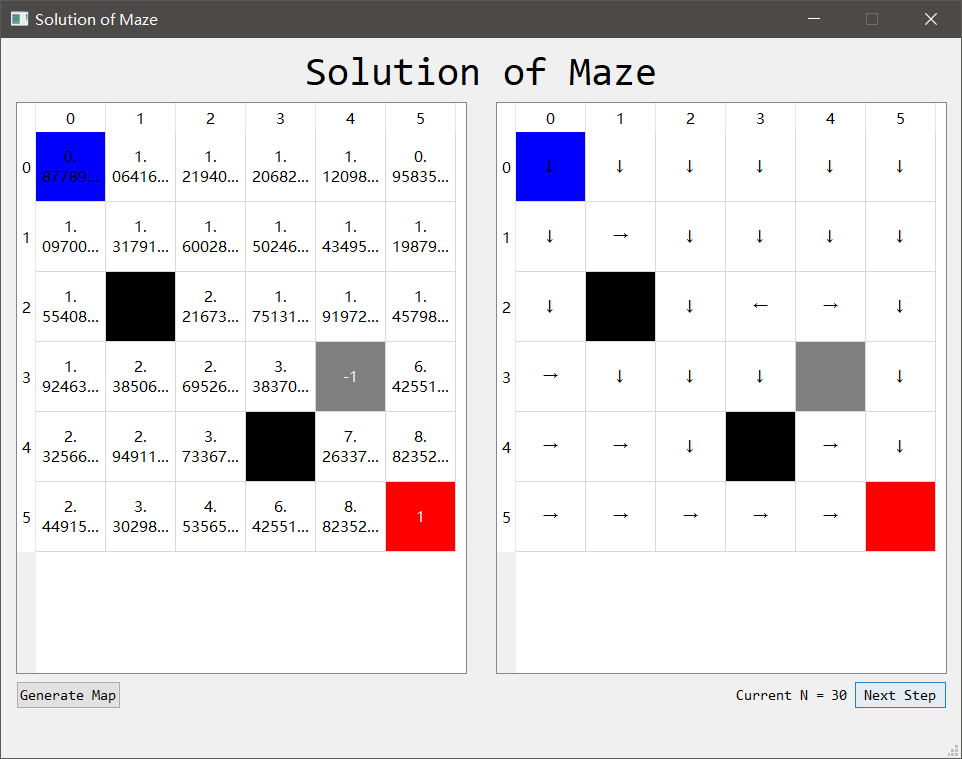
\includegraphics[width=0.4\textwidth]{figure4.png}
\end{figure}
\begin{figure}[H]
    \centering
    \caption{$N=40$}
    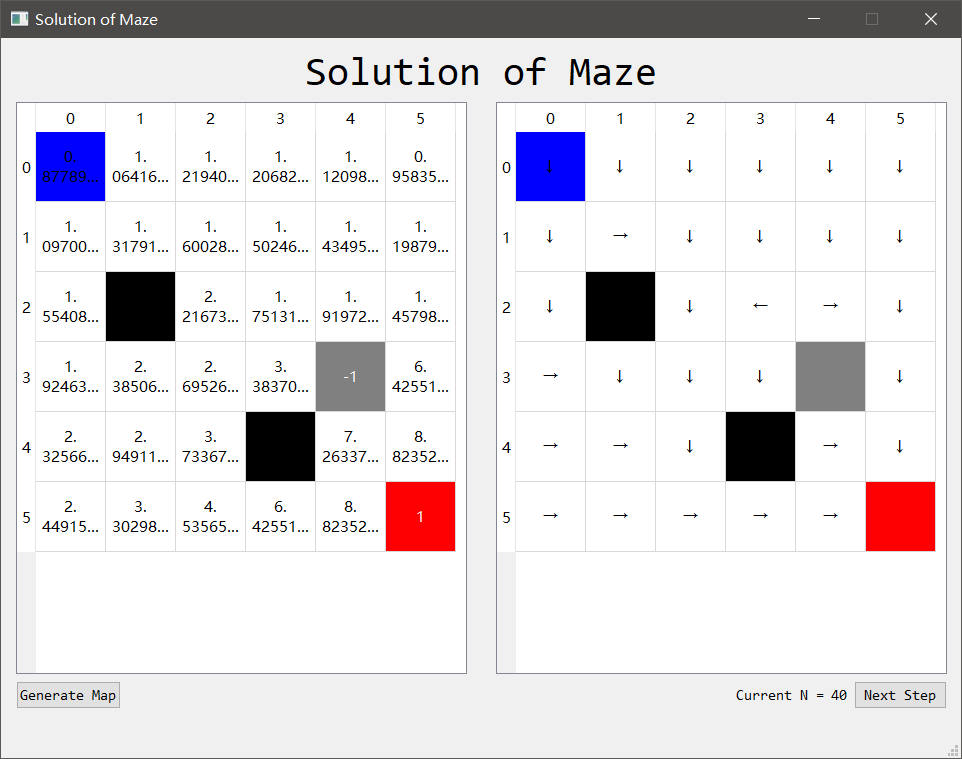
\includegraphics[width=0.4\textwidth]{figure5.png}
\end{figure}

可以看到, 执行到$N = 30$时, 价值已经收敛, 这时候右边的策略便是最优策略.

\section{实验感想}

本次实验实现的是一种比较简单的MDP, 找到的最优策略为确定性策略, 
而其他种类的MDP可能对应的是非确定性决策, 即$\pi(a|s)$可能对应的是非1值.
对于这种情况, 算法的迭代和最优策略的选取还需要修改. 
同时对于其他的MDP, 一次迭代收敛得到的价值函数未必对应的就是最优的策略, 这时候应该通过当前得到的最优策略, 
再次执行一次Bellman方程迭代过程, 然后再得出该步的最优策略, 重复, 直至得到收敛的最优策略.

MDP作为强化学习的一种基本方式, 是进入机器学习大门的必备知识点, 通过这次大作业, 对MDP的了解会更加深入.

\section{附录}
\subsection{UI使用说明}
UI采用PyQt库实现, 在运行时需要pip安装该库才能运行.\\ \\
运行方式:
\begin{lstlisting}
    python App.py
\end{lstlisting}
Solution界面:
\begin{itemize}
    \item Label: Current N 为当前N的值
    \item Button: Generate Map 点击以打开窗口属性设置 Setting 界面
    \item Button: Next Step 点击以进行下一次更新,此操作会刷新两个地图界面,同时使 Label: Current N ++
\end{itemize}
Setting界面:
\begin{itemize}
    \item Input: Size x/y 输入整数以设置地图大小
    \item Input: Traps 输入一组点坐标作为陷阱,不同点坐标间以一个空格(Space)分隔
    \item Input: Barriers 输入一组点坐标作为障碍,不同点坐标间以一个空格(Space)分隔
    \item Input: Start 输入一个点坐标作为起点
    \item Input: End 输入一组点坐标作为终点,不同点坐标间以一个空格(Space)分隔
    \item Button: Random 点击以随机生成上述参数,可在随机的结果上再做修改
    \item Button: Generate 点击以按照上述参数生成地图
\end{itemize}
% That's all folks!
\end{document}
